\section{Design of the Controller}\label{designController}

The root locus of the system with a proportional controller can be seen in \figref{rlocusCubli2}.

\begin{figure}[H]
	\centering 
	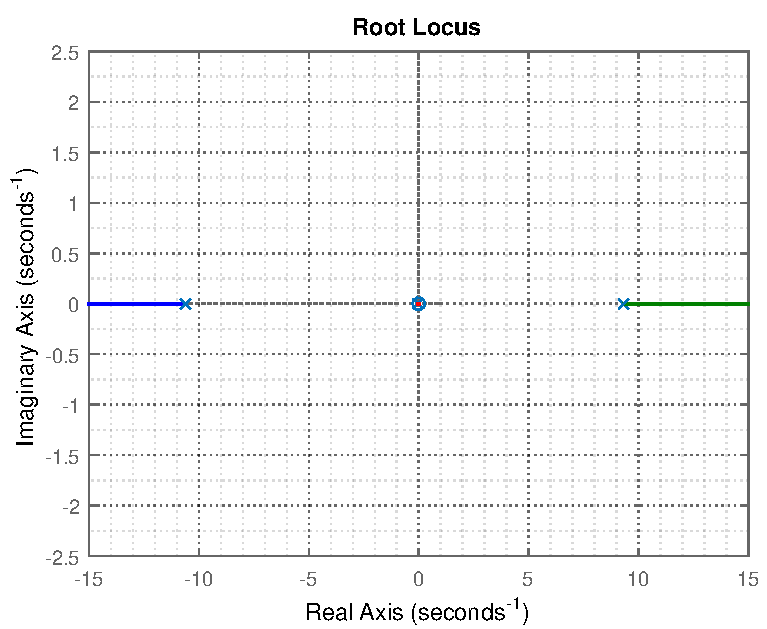
\includegraphics[scale=.75]{figures/rlocusCubli}
	\captionof{figure}{Root Locus of the system}
	\label{rlocusCubli2}
\end{figure}

Looking at the root locus it can be derived that the system can not be controlled using only a proportional controller because there is always a pole in the RHP no matter the gain.

However, a first approximation of the system's behavior in closed loop can be done through a proportional controller. Such a system is tested with a gain of 10 as a controller. The final closed loop poles are placed at \si{-40,4198,\ -0,0018\ and\ 39,2448}. In \figref{closedLoopResponse} it is shown the response of the simulation and the one from the real setup with this proportional controller.

\begin{figure}[H] 
	\centering 
	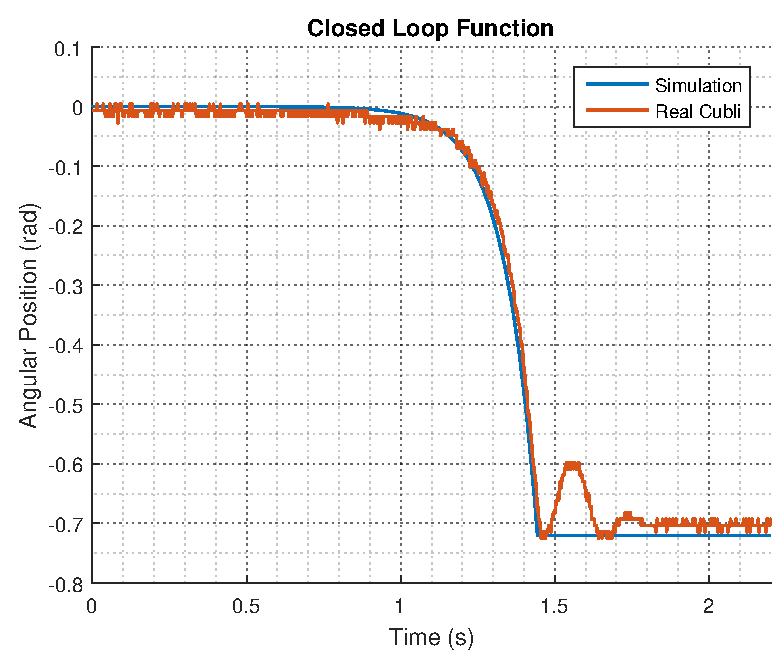
\includegraphics[scale=0.75]{figures/closedLoopResponse}	
	\caption{Behavior of the closed loop function with a proportional controller, both in simulation and reality}
	\label{closedLoopResponse}
\end{figure}
%
It is clear that, upon application of a \SI{0}{rad} reference and a minimal initial offset, the closed loop function with only a gain of 10 has an unstable response.
